\documentclass{standalone}
\usepackage{tikz}
\usetikzlibrary{patterns, positioning}
\usepackage[sfdefault]{ClearSans} %% option 'sfdefault' activates Clear Sans as the default text font
\usepackage[T1]{fontenc}

\begin{document}
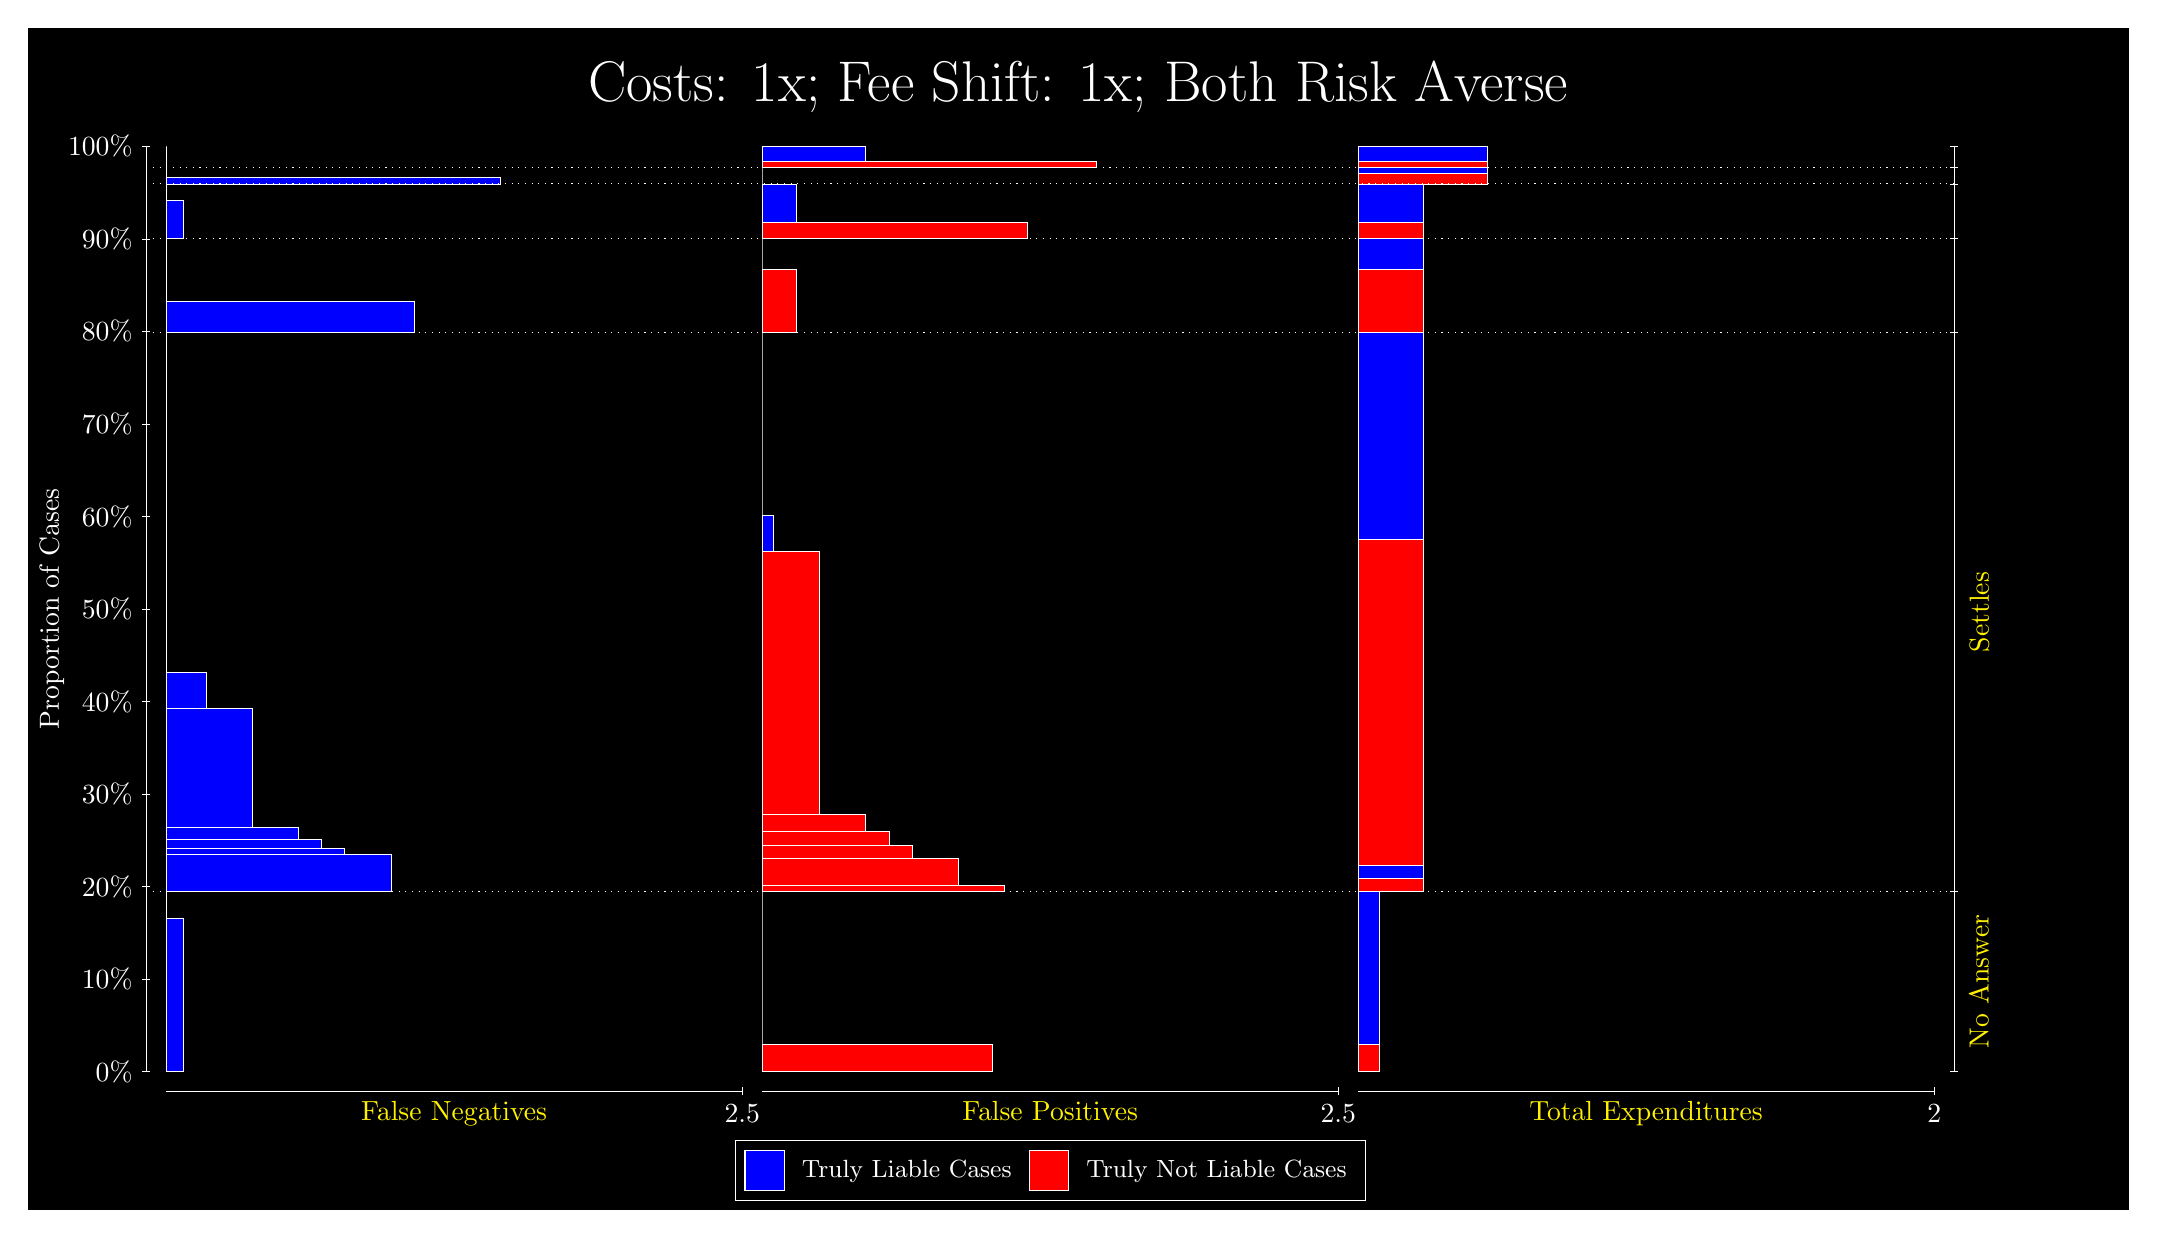
\begin{tikzpicture}
\draw[fill=black] (0,0) rectangle (26.667,15);
\draw[text=white] (0,13.5) rectangle (26.667,15) node[midway] {\huge Costs: 1x; Fee Shift: 1x; Both Risk Averse};
\draw[white, very thin] (1.5,1.75) -- (1.5,13.5);
\node[rotate=90, text=white, anchor=center] at (0.3, 7.625) {Proportion of Cases};
\draw[white, very thin] (1.45,1.75) -- (1.55,1.75);
\node[text=white, anchor=east] at (1.45, 1.75) {0\%};
\draw[white, very thin] (1.45,2.925) -- (1.55,2.925);
\node[text=white, anchor=east] at (1.45, 2.925) {10\%};
\draw[white, very thin] (1.45,4.1) -- (1.55,4.1);
\node[text=white, anchor=east] at (1.45, 4.1) {20\%};
\draw[white, very thin] (1.45,5.275) -- (1.55,5.275);
\node[text=white, anchor=east] at (1.45, 5.275) {30\%};
\draw[white, very thin] (1.45,6.45) -- (1.55,6.45);
\node[text=white, anchor=east] at (1.45, 6.45) {40\%};
\draw[white, very thin] (1.45,7.625) -- (1.55,7.625);
\node[text=white, anchor=east] at (1.45, 7.625) {50\%};
\draw[white, very thin] (1.45,8.8) -- (1.55,8.8);
\node[text=white, anchor=east] at (1.45, 8.8) {60\%};
\draw[white, very thin] (1.45,9.975) -- (1.55,9.975);
\node[text=white, anchor=east] at (1.45, 9.975) {70\%};
\draw[white, very thin] (1.45,11.15) -- (1.55,11.15);
\node[text=white, anchor=east] at (1.45, 11.15) {80\%};
\draw[white, very thin] (1.45,12.325) -- (1.55,12.325);
\node[text=white, anchor=east] at (1.45, 12.325) {90\%};
\draw[white, very thin] (1.45,13.5) -- (1.55,13.5);
\node[text=white, anchor=east] at (1.45, 13.5) {100\%};

\draw[white, very thin] (24.457,1.75) -- (24.457,13.5);
\draw[white, very thin] (24.407,1.75) -- (24.507,1.75);
\node[anchor=west] at (24.407, 1.75) {};
\draw[white, very thin] (24.407,4.0393) -- (24.507,4.0393);
\node[anchor=west] at (24.407, 4.0393) {};
\draw[white, very thin] (24.407,11.134) -- (24.507,11.134);
\node[anchor=west] at (24.407, 11.134) {};
\draw[white, very thin] (24.407,12.334) -- (24.507,12.334);
\node[anchor=west] at (24.407, 12.334) {};
\draw[white, very thin] (24.407,13.024) -- (24.507,13.024);
\node[anchor=west] at (24.407, 13.024) {};
\draw[white, very thin] (24.407,13.233) -- (24.507,13.233);
\node[anchor=west] at (24.407, 13.233) {};
\draw[white, very thin] (24.407,13.5) -- (24.507,13.5);
\node[anchor=west] at (24.407, 13.5) {};

\draw[white, very thin, fill=blue] (1.75,1.75) rectangle (1.9696,3.694);
\draw[white, very thin, fill=red] (1.75,3.694) rectangle (1.75,4.0393);
\draw[white, very thin, fill=blue] (1.75,4.0393) rectangle (4.6044,4.5116);
\draw[white, very thin, fill=blue] (1.75,4.5116) rectangle (4.0188,4.5873);
\draw[white, very thin, fill=blue] (1.75,4.5873) rectangle (3.7261,4.6982);
\draw[white, very thin, fill=blue] (1.75,4.6982) rectangle (3.4333,4.8554);
\draw[white, very thin, fill=blue] (1.75,4.8554) rectangle (2.8478,6.3582);
\draw[white, very thin, fill=blue] (1.75,6.3582) rectangle (2.2623,6.8219);
\draw[white, very thin, fill=red] (1.75,6.8219) rectangle (1.75,11.134);
\draw[white, very thin, fill=blue] (1.75,11.134) rectangle (4.8971,11.53);
\draw[white, very thin, fill=red] (1.75,11.53) rectangle (1.75,12.334);
\draw[white, very thin, fill=blue] (1.75,12.334) rectangle (1.9696,12.819);
\draw[white, very thin, fill=red] (1.75,12.819) rectangle (1.75,13.024);
\draw[white, very thin, fill=blue] (1.75,13.024) rectangle (5.9949,13.103);
\draw[white, very thin, fill=red] (1.75,13.103) rectangle (1.75,13.233);
\draw[white, very thin, fill=red] (1.75,13.233) rectangle (1.75,13.312);
\draw[white, very thin, fill=blue] (1.75,13.312) rectangle (1.75,13.5);
\draw[white, very thin, fill=red] (9.3189,1.75) rectangle (12.246,2.0953);
\draw[white, very thin, fill=blue] (9.3189,2.0953) rectangle (9.3189,4.0393);
\draw[white, very thin, fill=red] (9.3189,4.0393) rectangle (12.393,4.1127);
\draw[white, very thin, fill=red] (9.3189,4.1127) rectangle (11.807,4.4544);
\draw[white, very thin, fill=red] (9.3189,4.4544) rectangle (11.222,4.6224);
\draw[white, very thin, fill=red] (9.3189,4.6224) rectangle (10.929,4.8026);
\draw[white, very thin, fill=red] (9.3189,4.8026) rectangle (10.636,5.0185);
\draw[white, very thin, fill=red] (9.3189,5.0185) rectangle (10.051,8.3514);
\draw[white, very thin, fill=blue] (9.3189,8.3514) rectangle (9.4652,8.8151);
\draw[white, very thin, fill=blue] (9.3189,8.8151) rectangle (9.3189,11.134);
\draw[white, very thin, fill=red] (9.3189,11.134) rectangle (9.758,11.938);
\draw[white, very thin, fill=blue] (9.3189,11.938) rectangle (9.3189,12.334);
\draw[white, very thin, fill=red] (9.3189,12.334) rectangle (12.686,12.539);
\draw[white, very thin, fill=blue] (9.3189,12.539) rectangle (9.758,13.024);
\draw[white, very thin, fill=red] (9.3189,13.024) rectangle (9.3189,13.153);
\draw[white, very thin, fill=blue] (9.3189,13.153) rectangle (9.3189,13.233);
\draw[white, very thin, fill=red] (9.3189,13.233) rectangle (13.564,13.312);
\draw[white, very thin, fill=blue] (9.3189,13.312) rectangle (10.636,13.5);
\draw[white, very thin, fill=red] (16.888,1.75) rectangle (17.162,2.0953);
\draw[white, very thin, fill=blue] (16.888,2.0953) rectangle (17.162,4.0393);
\draw[white, very thin, fill=red] (16.888,4.0393) rectangle (17.711,4.2073);
\draw[white, very thin, fill=blue] (16.888,4.2073) rectangle (17.711,4.3645);
\draw[white, very thin, fill=red] (16.888,4.3645) rectangle (17.711,8.5086);
\draw[white, very thin, fill=blue] (16.888,8.5086) rectangle (17.711,11.134);
\draw[white, very thin, fill=red] (16.888,11.134) rectangle (17.711,11.938);
\draw[white, very thin, fill=blue] (16.888,11.938) rectangle (17.711,12.334);
\draw[white, very thin, fill=red] (16.888,12.334) rectangle (17.711,12.539);
\draw[white, very thin, fill=blue] (16.888,12.539) rectangle (17.711,13.024);
\draw[white, very thin, fill=red] (16.888,13.024) rectangle (18.534,13.153);
\draw[white, very thin, fill=blue] (16.888,13.153) rectangle (18.534,13.233);
\draw[white, very thin, fill=red] (16.888,13.233) rectangle (18.534,13.312);
\draw[white, very thin, fill=blue] (16.888,13.312) rectangle (18.534,13.5);
\draw[white, dotted] (1.5,4.0393) -- (24.457,4.0393);
\draw[white, dotted] (1.5,11.134) -- (24.457,11.134);
\draw[white, dotted] (1.5,12.334) -- (24.457,12.334);
\draw[white, dotted] (1.5,13.024) -- (24.457,13.024);
\draw[white, dotted] (1.5,13.233) -- (24.457,13.233);
\draw[white, very thin] (1.75,1.5) -- (9.0689,1.5);
\node[text=yellow, anchor=north] at (5.4094, 1.5) {False Negatives};
\draw[white, very thin] (9.0689,1.45) -- (9.0689,1.55);
\node[text=white, anchor=north] at (9.0689, 1.45) {2.5};

\draw[white, very thin] (9.3189,1.5) -- (16.638,1.5);
\node[text=yellow, anchor=north] at (12.978, 1.5) {False Positives};
\draw[white, very thin] (16.638,1.45) -- (16.638,1.55);
\node[text=white, anchor=north] at (16.638, 1.45) {2.5};

\draw[white, very thin] (16.888,1.5) -- (24.207,1.5);
\node[text=yellow, anchor=north] at (20.547, 1.5) {Total Expenditures};
\draw[white, very thin] (24.207,1.45) -- (24.207,1.55);
\node[text=white, anchor=north] at (24.207, 1.45) {2};

\node[text=yellow, centered, rotate=90] at (24.777, 2.8947) {No Answer};
\node[text=yellow, centered, rotate=90] at (24.777, 7.5866) {Settles};





\draw (12.978300999999998,1.5) node[draw=none] (baseCoordinate) {};
\begin{scope}[align=center]
        \matrix[scale=0.5, draw=white, below=0.5cm of baseCoordinate, nodes={draw}, column sep=0.1cm]{
            \node[rectangle, draw, minimum width=0.5cm, minimum height=0.5cm, fill=blue] {}; &
            \node[draw=none, font=\small, text=white] (B) {Truly Liable Cases}; &
            \node[rectangle, draw, minimum width=0.5cm, minimum height=0.5cm, fill=red] {}; &
            \node[draw=none, font=\small, text=white] (B) {Truly Not Liable Cases}; \\
            };
\end{scope}

\end{tikzpicture}
\end{document}